\documentclass[11pt]{article}

\usepackage[french, english]{babel}

\usepackage[T1]{fontenc}

\usepackage{amsfonts}
\usepackage{amsmath}
\usepackage{amssymb}

\usepackage{graphicx}
\usepackage{multirow}
\usepackage{multicol}
\usepackage{xcolor}
\usepackage[shortlabels]{enumitem}

\usepackage[margin=2cm]{geometry}

\usepackage{mathtools}
\usepackage{siunitx}
\usepackage{braket}

\usepackage{listings}

\usepackage{tikz}
\usetikzlibrary{shapes.geometric, arrows.meta, positioning, calc}

\tikzstyle{block} = [rectangle, rounded corners, minimum width=4cm, minimum height=1cm,
text centered, draw=black, fill=blue!10]
\tikzstyle{process} = [rectangle, rounded corners, minimum width=5cm, minimum height=1cm,
text centered, draw=black, fill=green!10]
\tikzstyle{io} = [trapezium, trapezium left angle=70, trapezium right angle=110,
minimum width=4cm, minimum height=1cm, text centered, draw=black, fill=orange!15]
\tikzstyle{decision} = [diamond, aspect=2, draw=black, fill=yellow!15, text centered]
\tikzstyle{arrow} = [thick, ->, >=Stealth]

\renewcommand\lstlistingname{Code Python}

\lstset{frame=tb,
  language=Python,
  numbers=left,
  stepnumber=1,
  aboveskip=3mm,
  belowskip=3mm,
  showstringspaces=false,
  columns=flexible,
  basicstyle={\small\ttfamily},
%   numbers=none,
  numberstyle=\tiny\color{gray},
  keywordstyle=\color{blue},
  commentstyle=\color{paired2b},
  stringstyle=\color{paired3b},
  breaklines=true,
  breakatwhitespace=true,
  tabsize=1,
  frame=single,
%   showtabs=false,
}


\begin{document}

\renewcommand*{\contentsname}{Table des matières}

\hrule

\begin{center}
  {\Large GEI299 - Gestion de projet} \\ \vspace{5mm}
  {\LARGE\sffamily Planification du projet} \\
  Alexis Jean\\
  À remettre le 20 novembre 2025
\end{center}

\hrule

\tableofcontents

\hrule

\section{\underline{Introduction}}
La compagnie GE Healthcare a mandaté notre équipe pour le développement d'un logiciel visant à trouver de meilleurs candidats que le gadolinium dans le cadre de l'imagerie par résonance magnétique (IRM). Le but principal du projet est de concevoir un logiciel capable d'analyser et de comparer différents composés chimiques afin d'identifier ceux qui pourraient servir d'agents de contraste plus efficaces et plus sûrs que le gadolinium actuellement utilisé.


\section{\underline{Survol du projet}}
Le projet consiste à développer un logiciel pour effectuer des simulations quantiques dans le but de simuler les états fondamentaux ainsi que les propriétés électroniques des différents candidats possibles. Les livrables sont un rapport technique, un cahier Jupyter ainsi qu'une présentation de haut niveau pour des gens d'affaires. Le tout doit être livré au bout de 2 mois avec un budget d'au plus 200 000\$ CAD.


\section{\underline{Structure organisationnelle du projet}}
Dans cette section, on présente la hiérarchie de l'équipe dans le cadre du projet. Le diagramme suivant décrit la dite structure :

\newpage

\subsection{Schéma de la hiérarchie}

\begin{figure}[h!]
  \centering
  \begin{tikzpicture}[node distance=2cm]

    \node (client) [block] {GE Healthcare};
    \node (chef) [block] [below of=client]{Chef de projet};
    \node (inge) [block] [below of=chef, xshift=0cm] {Ingénieur logiciel};
    \node (fin) [block, below of=chef, xshift=-4cm] {Chargé financier};
    \node (log) [block, below of=chef, xshift=4cm] {Logistique};
    
    \tikzset{smallblock/.style={block, minimum width=2cm, minimum height=0.8cm, font=\small}}
    
    \node (elog) [smallblock, below of=inge, xshift=-6.5cm] {Équipe logiciel};
    \node (eelec) [smallblock, below of=inge, xshift=-3.5cm] {Équipe électronique};
    \node (etest) [smallblock, below of=inge, xshift=7.25cm] {Équipe test \& calibration};
    \node (esci) [smallblock, below of=inge, xshift=3.5cm] {Équipe scientifique};
    \node (edoc) [smallblock, below of=fin, xshift=4cm] {Équipe documentation};
    
    \draw [arrow] (client) -- (chef);
    \draw [arrow] (chef) -- (inge);
    \draw [arrow] (chef) -- (fin);
    \draw [arrow] (chef) -- (log);
    \draw [arrow] (inge) -- (elog);
    \draw [arrow] (inge) -- (eelec);
    \draw [arrow] (inge) -- (etest);
    \draw [arrow] (inge) -- (esci);
    \draw [arrow] (inge) -- (edoc);

  \end{tikzpicture}
  \caption{Structure organisationnelle du projet}
\end{figure}

\subsection{Description des rôles}

\begin{itemize}
  \item \textbf{Client} : GE Healthcare est le client principal du projet. Ils fournissent les exigences et les ressources nécessaires pour le développement du logiciel.
  \item \textbf{Chef de projet} : Responsable de la planification, de l'exécution et de la clôture du projet. Il coordonne les différentes équipes et assure la communication avec le client.
  \item \textbf{Ingénieur logiciel} : Supervise le développement logiciel, s'assure que les exigences techniques sont respectées et coordonne les équipes techniques.
  \item \textbf{Chargé financier} : Gère le budget du projet, surveille les dépenses et s'assure que le projet reste financièrement viable.
  \item \textbf{Logistique} : Responsable de la gestion des ressources matérielles, de l'approvisionnement et de la distribution des équipements nécessaires au projet.
  \item \textbf{Équipes spécialisées} : Chaque équipe (logiciel, électronique, test \& calibration, scientifique, documentation) est responsable de ses tâches spécifiques dans le cadre du projet.
\end{itemize}

\newpage

\section{\underline{Répartition des rôles et responsabilités}}
Dans la section qui suit, on décrit les rôles ainsi que les responsabilités de chaque entité de la hiérarchie illustrée plus tôt.

\begin{itemize}
  \item \textbf{Client (GE Healthcare)} :
    \begin{itemize}
      \item Fournir les exigences du projet.
      \item Valider les livrables.
      \item Offrir un soutien financier et logistique.
    \end{itemize}
  \item \textbf{Chef de projet} :
    \begin{itemize}
      \item Planifier et organiser les activités du projet.
      \item Gérer les ressources humaines et matérielles.
      \item Assurer la communication entre les équipes et le client.
      \item Suivre l'avancement du projet et gérer les risques.
    \end{itemize}
  \item \textbf{Ingénieur logiciel} :
    \begin{itemize}
      \item Superviser le développement technique du logiciel.
      \item Assurer la conformité aux normes de qualité.
      \item Coordonner les efforts des équipes techniques.
    \end{itemize}
  \item \textbf{Chargé financier} :
    \begin{itemize}
      \item Élaborer et gérer le budget du projet.
      \item Surveiller les coûts et les dépenses.
      \item Préparer des rapports financiers pour le chef de projet.
    \end{itemize}
  \item \textbf{Logistique} :
    \begin{itemize}
      \item Gérer l'approvisionnement en matériel et équipements.
      \item Coordonner la distribution des ressources aux équipes.
      \item Assurer la maintenance des équipements utilisés dans le projet.
    \end{itemize}
  \item \textbf{Équipes spécialisées} :
    \begin{itemize}
      \item Chaque équipe est responsable de la réalisation de ses tâches spécifiques, telles que le développement logiciel, la conception électronique, les tests et calibrations, la recherche scientifique, et la documentation technique.
    \end{itemize}
\end{itemize}

\newpage

\section{\underline{Planification du travail}}
Cette section traite de la planification du travail avec un diagramme réseau AON ainsi qu'un diagramme de Gantt illustrant les différentes tâches, leurs dépendances, et la durée estimée pour chaque tâche.

\subsection{Schéma réseau AON}
On présente ici le diagramme réseau AON sur la page suivante avec la légende des tâches et leur durée respective. Les détails de chaque tâche sont fournis après les diagrammes.

\begin{itemize}
  \item T1 : Dépendances (1 semaine)
  \item T2 : Architecture (1 semaine)
  \item T3 : Design de l'interface (1 semaine)
  \item T5 : Schématisation (2 semaines)
  \item T9 : Assemblage (1 semaine)
  \item T10 : Tests unitaires (1 semaine)
  \item T11 : Intégration (2 semaines)
  \item T12 : Calibration (1 semaine)
  \item T13 : Validation et tests finaux (1 semaine)
  \item T14a : Brouillon documentation (1 semaine)
  \item T14b : Documentation finale (1 semaine)
  \item T15 : Projet rendu (1 semaine)
  \item Rouge : Tâches critiques
  \item Bleu : Tâches non critiques
\end{itemize}

\newpage 

\begin{tikzpicture}[node distance=18mm and 12mm, >=Latex]
  \tikzset{
    task/.style={rectangle, draw=black, rounded corners=4pt, fill=blue!6, inner sep=6pt, align=center, font=\small},
    taskcrit/.style={rectangle, draw=red!80, rounded corners=4pt, fill=red!6, inner sep=6pt, align=center, font=\small},
    arrow/.style={-Stealth, thick}
  }

  % niveau 1
  \node[taskcrit] (T1) {T1\\Dépendances\\(1s)};

  % niveau 2
  \node[taskcrit, below=of T1] (T2a) {T2a\\Architecture\\(1s)};
  \node[task, right=14mm of T1, xshift=6.6cm] (T2b) {T2b\\Design de l'interface\\(1s)};

  % niveau 3
  \node[taskcrit, below=of T2a] (T3) {T3\\Schématisation\\(2s)};
  \node[task, below=of T2b] (T9a) {T9a\\Brouillon docu\\(1s)};

  % niveau 4
  \node[taskcrit, below=of T3, xshift=8cm] (T5) {T5\\Tests unitaires\\(1s)};
  \node[taskcrit, below=of T3] (T4) {T4\\Assemblage\\(1s)};

  % niveau 5 - intégration
  \node[taskcrit] (T6) at ($(T4)!0.5!(T5)$) {T6\\Intégration\\(2s)};
  \node[taskcrit, below=of T6] (T7) {T7\\Calibration\\(1s)};
  \node[taskcrit, below=of T7] (T8) {T8\\Validation et tests finaux\\(1s)};

  % docs final + livraison
  \node[taskcrit, right=of T8, xshift=26mm] (T9b) {T9b\\Docu finale\\(1s)};
  \node[taskcrit, below=of T8, xshift=20mm] (T10) {T10\\Projet rendu\\(1s)};

  \draw[arrow] (T1) -- (T2a);
  \draw[arrow] (T1) -- (T2b);

  \draw[arrow] (T2a) -- (T3);

  
  \draw [arrow] (T3) -- (T4);
  \draw[arrow] (T3) -- (T5);

  \draw[arrow] (T4) -- (T6);
  \draw[arrow] (T5) -- (T6);

  \draw[arrow] (T6) -- (T7);
  \draw[arrow] (T7) -- (T8);

  \draw[arrow] (T8) -- (T9b);
  \draw[arrow] (T9b) -- (T10);
  \draw[arrow] (T8) -- (T10);

  \draw[arrow,dashed] (T2b) -- (T9a);
  \draw[arrow,dashed] (T9a) -- (T9b);

\end{tikzpicture}

\newpage

\subsection{Diagramme de Gantt}
Dans cette section, on présente la planification du projet sous la forme de diagramme de Gantt.
\begin{figure}[h!]
  \centering
  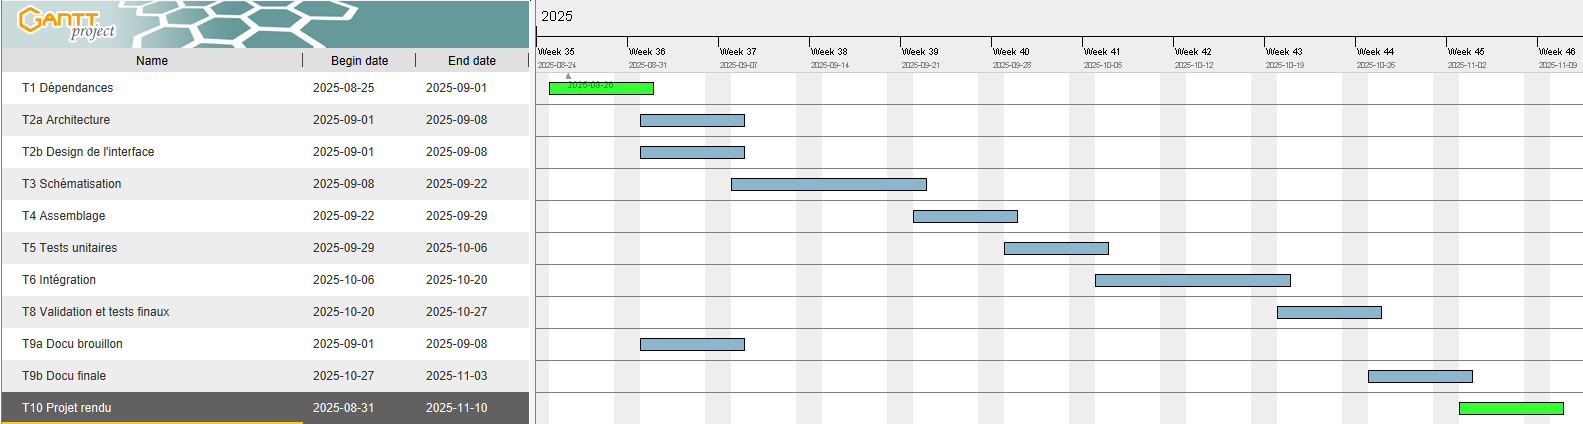
\includegraphics[width=\textwidth]{gantt.png}
  \caption{Diagramme de Gantt du projet}
\end{figure}

\begin{itemize}
  \item \textbf{T1 Dépendances :} Il s'agit de la première tâche du projet, qui consiste à identifier et analyser les dépendances entre les différentes tâches et ressources nécessaires pour mener à bien le projet.
  \item \textbf{T2a Architecture :} L'ingénieur logiciel conçoit le plan de l'architecture du logiciel, en d'autres mots, comment chaque partie du logiciel va interagir.
  \item \textbf{T2b Design de l'interface :} Cette tâche consiste à créer le design de l'interface utilisateur du logiciel, en s'assurant qu'elle soit intuitive et facile à utiliser.
  \item \textbf{T3 Schématisation :} Cette tâche implique la création de schémas détaillés du logiciel, y compris les diagrammes de flux de données et les diagrammes de structure.
  \item \textbf{T4 Assemblage :} Cette tâche consiste à assembler les différentes parties du logiciel, en intégrant les modules développés par les différentes équipes.
  \item \textbf{T5 Tests unitaires :} Chaque module du logiciel est testé individuellement pour s'assurer qu'il fonctionne correctement.
  \item \textbf{T6 Intégration :} Les modules testés sont intégrés ensemble pour former le logiciel.
  \item \textbf{T7 Calibration :} Le logiciel est calibré pour s'assurer qu'il fonctionne correctement avec les différents candidats.
  \item \textbf{T8 Validation et tests finaux :} Le logiciel est soumis à des tests finaux pour valider son bon fonctionnement et sa conformité aux exigences du client.
  \item \textbf{T9a Brouillon documentation :} Un brouillon de la documentation technique du logiciel est créé, incluant les instructions d'utilisation et les spécifications techniques.
  \item \textbf{T9b Documentation finale :} La documentation technique est finalisée et prête à être livrée avec le logiciel.
  \item \textbf{T10 Projet rendu :} Le projet est officiellement rendu au client, ayant le logiciel ainsi que les livrables prévus.
\end{itemize}


\newpage

\section{\underline{Évaluation et gestion des coûts}}
La gestion du budget est proposée par ce tableau qui illustre les coûts estimés pour chaque mois du projet, répartis en trois catégories principales : personnel, services et dépenses diverses et ce, sur une période de 4 mois en accord avec la planification du travail comme identifié plus tôt.

\begin{table}[h!]
\centering
\caption{Évaluation des coûts du projet pour chaque mois}
\resizebox{\textwidth}{!}{\begin{tabular}{lcccccccc}
\hline
 & \multicolumn{2}{c}{Août} & \multicolumn{2}{c}{Septembre} 
 & \multicolumn{2}{c}{Octobre} & \multicolumn{2}{c}{Novembre} \\
 & Jours/Min & k\$ & Jours/Min & k\$ & Jours/Min & k\$ & Jours/Min & k\$ \\
\hline
\textbf{Personnel} \\
Stagiaires (2)                  & -- & 2.25 & -- & 2.25 & -- & 2.25 & -- & 2.25 \\
Chimiste (1000/jour)            & 4  & 4.0  & 5  & 5.0  & 4  & 4.0  & 2  & 2.0 \\
Personnel de recherche          & 3  & 3.0  & 3  & 3.0  & 2  & 2.0  & 2  & 2.0 \\
\textit{Sous-total}             &    & \textbf{9.25} 
                                &    & \textbf{10.25} 
                                &    & \textbf{8.25} 
                                &    & \textbf{6.25} \\
\\
\textbf{Services} \\
Accès IBM Quantum (48/min)      & 300 & 14.4 & 400 & 19.2 & 300 & 14.4 & 200 & 9.6 \\
Bureau de dessin (300/jour)     & 2   & 0.6  & 2   & 0.6  & 1   & 0.3  & --  & 0.0 \\
Atelier prototype (350/jour)    & --  & 0.0  & 4   & 1.4  & 4   & 1.4  & 2   & 0.7 \\
\textit{Sous-total}             &     & \textbf{15.0}
                                &     & \textbf{21.2}
                                &     & \textbf{16.1}
                                &     & \textbf{10.3} \\
\\
\textbf{Dépenses} \\
Matériaux                       & -- & 2.0 & -- & 1.5 & -- & 1.0 & -- & 0.5 \\
Autres                          & -- & 1.0 & -- & 0.5 & -- & 0.3 & -- & 0.2 \\
\textit{Sous-total}             &    & \textbf{3.0}
                                &    & \textbf{2.0}
                                &    & \textbf{1.3}
                                &    & \textbf{0.7} \\
\hline
\textbf{TOTAL}                  &    & \textbf{27.25}
                                &    & \textbf{33.45}
                                &    & \textbf{25.65}
                                &    & \textbf{17.25} \\
\hline
\end{tabular}}
\end{table}



\end{document}







